\documentclass[11pt]{amsart}
\usepackage[margin=2.5cm]{geometry}                % See geometry.pdf to learn the layout options. There are lots.
\geometry{letterpaper}                   % ... or a4paper or a5paper or ...
%\geometry{landscape}                % Activate for for rotated page geometry
%\usepackage[parfill]{parskip}    % Activate to begin paragraphs with an empty line rather than an indent
\usepackage{algorithm}
\usepackage[noend]{algpseudocode}
\usepackage{graphicx}
\usepackage{amssymb,amsfonts}
\usepackage{epstopdf}
\usepackage{multicol}
\DeclareGraphicsRule{.tif}{png}{.png}{`convert #1 `dirname #1`/`basename #1 .tif`.png}

\title{Evacuating Priority Agents in a Disk with Unknown Exit Location}
\author{David Bushta, Christopher Till, Sunil Shende}
%\date{}                                           % Activate to display a given date or no date

\begin{document}
\maketitle
\section{Preliminaries}

Algorithms of search-and-escape involve mobile agents (also called Robots)
searching in geometric domains, such as a closed disk, or convex polygon. By
working together and communicating with one another, these mobile agents search
the domain to find an exit hidden on the perimeter. Many different problems have
previously been studied in this topic, such as finding algorithms to evacuate all
agents in a domain, or only evacuating a specific subset of these agents.

\subsection{Model}


All agents in this problem use the same coordinate system and operate in a closed
disk, all starting from the center. These agents' algorithms do not all have to be the same,
and in fact to most efficiently search the circle, they must all be unique.
In our problem, we observe the Priority model of algorithms. In this model, a
subset of one or more agents (P) are defined as a Priority (or Queen) and the goal
of the algorithm is to evacuate a required subset of these Priority Agents. These
algorithms also include a number Helper agents (H), that simply assist in searching the circle
for the exit, for a total of (H + P) agents. The Helper agents are not required to evacuate.


Once an exit is found, whether by a Helper or a Priority, the agent may use
Wireless communication to immediately broadcast the exit's location and its own identity to all other agents.
Upon receiving this broadcasted location, any remaining Priority agents that
need to evacuate travel along a chord to the exit and when the required subset has exited, the algorithm terminates.
The cost of the algorithm is called the termination time, and is the total worst-case
time for the required subset of Priority agents to exit.

\subsection{Previous Work}

Similar search-and-evacuate problems to this one have previously been studied, including those involving Agents
searching on a line, and searching inside of other types of shapes, such as a triangle.
In our research thus far, we have mainly looked at the problems regarding
the closed unit disk and how to most efficiently search for the exit and evacuate
different subsets of agents. We started by studying the algorithms that have been designed
for $n = 2, 3$ agents using both the face-to-face and wireless communication models [(Evacuating Robots
From a Disk Using Face-to-Face Communication, 2015), (Evacuating Robots Via an Unknown Exit in a Disk, 2015)].
In these algorithms, all agents must evacuate for the algorithm to terminate, and there is no notion of
Priority of Helper. Interestingly, in the face-to-face model, agents must be next to each other to
communicate.


Afterwards, we looked at problems of a similar type that have been studied,
namely those regarding 1 Priority and 1 or more Helper agents searching in a
closed disk solely usign wireless communication (God Save the Queen, 2018)
(Priority Evacuation From a Disk Using Mobile Robots, 2018)].
In these papers, the results involved getting the only Priority agent to the exit
as fast as possible, however, our problem attempts to design an algorithm where
only one of multiple Priority agents needs to evacuate.


To facilitate studying these algorithms and seeing results based on test data, we
have created an algorithm visualizer. This program uses the different types of movement and
communication directives we commonly see in each algorithm to recreate an
interactive visualization of the algorithm. To date, all of the algorithms
listed in the above papers including our own can be shown, and new ones can be created.


\subsection{Our Results}

In our algorithm using 2 Priority and 1 Helper agent with 1 Priority required to exit, we show that a termination time
upper bound of \textbf{3.55 time units} is possible given the specific set of parameters we use
to guide the agents. We can achieve this by using a \textbf{parameter of angle $\alpha = 5 \pi / 9 - 2\sqrt3 /3$} for the two agents to travel to the perimeter in the third quadrant, i.e, they travel out at
an angle of \textbf{$\pi + \alpha$}. This allows us to set the two worst-case time predictions equal.
These are the cases where \textbf{$A)$} $P2$ finds the exit at the very end of its search,
or \textbf{$B)$} $H$ finds the exit in the second quadrant at the angle \textbf{$\pi - \beta$},
where \textbf{$\beta = ( \pi / 3 - \alpha) / 2$}.




\section{Algorithm 1}

%Our first priority algorithm with 2 queens and 1 servant

\begin{algorithm}
  \caption{Priority and Helper Algorithm}
  \begin{algorithmic}[1]
    \Procedure{Search}{$\alpha$}\Comment{Search for exit and evacuate closest Priority}
      \State $P1, P2, H$ are 2 Priority and Helper respectively.
      \State All angles are on the typical unit circle.
      \State $P1$ goes to the perimeter of the disk at angle 0.
      \State $P2$ and $H$ go to the perimeter at angle ($\pi$ + $\alpha$).
      \Repeat $P1$ and $H$ travel clockwise and $P2$ travels counterclockwise \Until{Exit is found.}
      \If {$H$ Finds the exit} $H$ broadcasts the exit location, and the closer of the
      two ($P1$ or $P2$) travels along a chord directly to the exit. The algorithm then terminates. \EndIf
      \If {$P1$ or $P2$ finds the exit} the algorithm terminates. \EndIf
    \EndProcedure
  \end{algorithmic}
\end{algorithm}

\includegraphics{mypics/2Q1S_Initial.pdf}
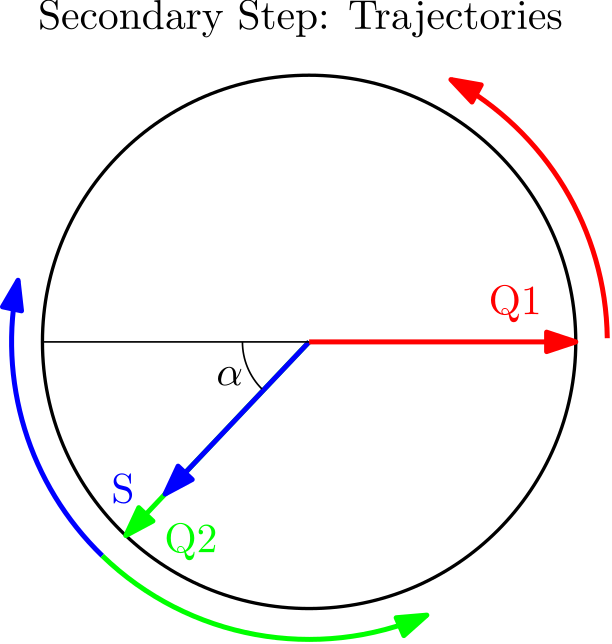
\includegraphics{mypics/2Q1S_Second_Step.pdf}
% \includegraphics{mypics/2Q1S_Initial.pdf}
% \includegraphics{mypics/2Q1S_Initial.pdf}

\end{document}
